% buscar en el genbank de mbi

\begin{frame}
\begin{center}
	\Huge{Genoma}
\end{center}
\end{frame}


\begin{frame}
\frametitle{Genoma}
\framesubtitle{¿Qué es?}
\begin{itemize}
    \item \textbf{Totalidad} de la información genética que posee un organismo en
		particular.
    \begin{itemize}
        \item No olviden al genoma Mitocondrial!
    \end{itemize}
\end{itemize}
\begin{center}
	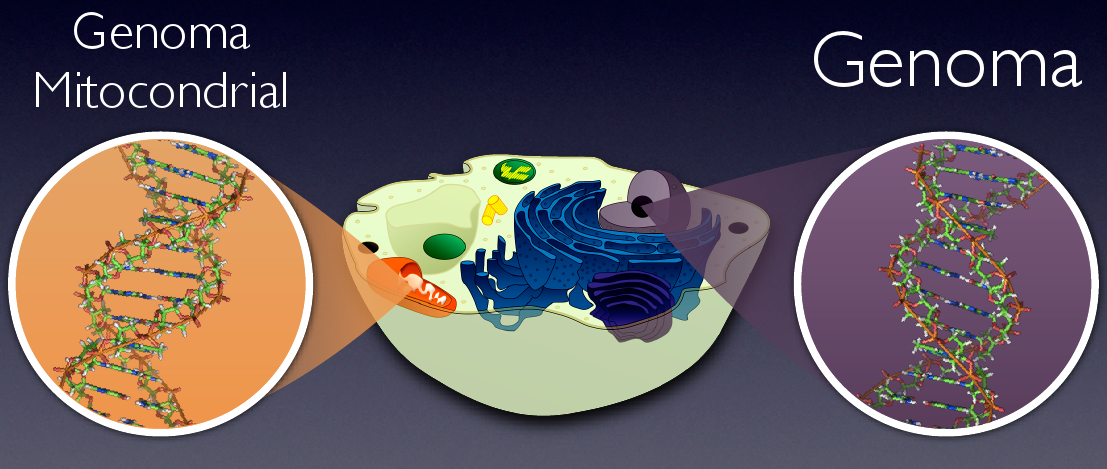
\includegraphics[width=0.9\textwidth]{img/genomas}
\end{center}
\end{frame}


\begin{frame}
\frametitle{Genoma}
\framesubtitle{¿Qué contiene?}
\begin{columns}
\begin{column}{0.7\textwidth}
	\begin{itemize}
	    \item \textbf{Genes} que codifican \textbf{proteínas}.
	    \item ``Genes'' que codifican \textbf{RNA's estructurales}: rRNA, tRNA, etc.
	    \item Secuencias de \textbf{control}.
	    \item En general, mucha \textbf{basura}.
	    \begin{itemize}
	        \item Repeticiones de secuencias.
	        \item Hartas A y T (en relación a la estructura de la cromatina).
	        \item Duplicados en desuso.
	        \item Minisatélites, Microsatélites.
	        \item Largo etc.
	    \end{itemize}
	\end{itemize}
\end{column}
\begin{column}{0.3\textwidth}
	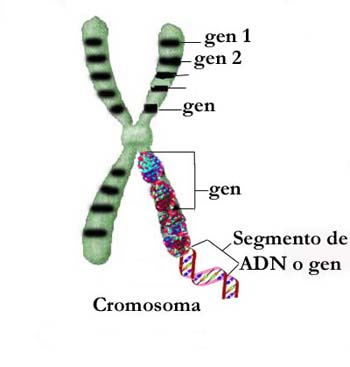
\includegraphics[width=0.95\textwidth]{img/gen.jpg}
\end{column}
\end{columns}
\end{frame}

\begin{frame}
\frametitle{Genoma}
\framesubtitle{¿Qué contiene?}
\begin{center}
	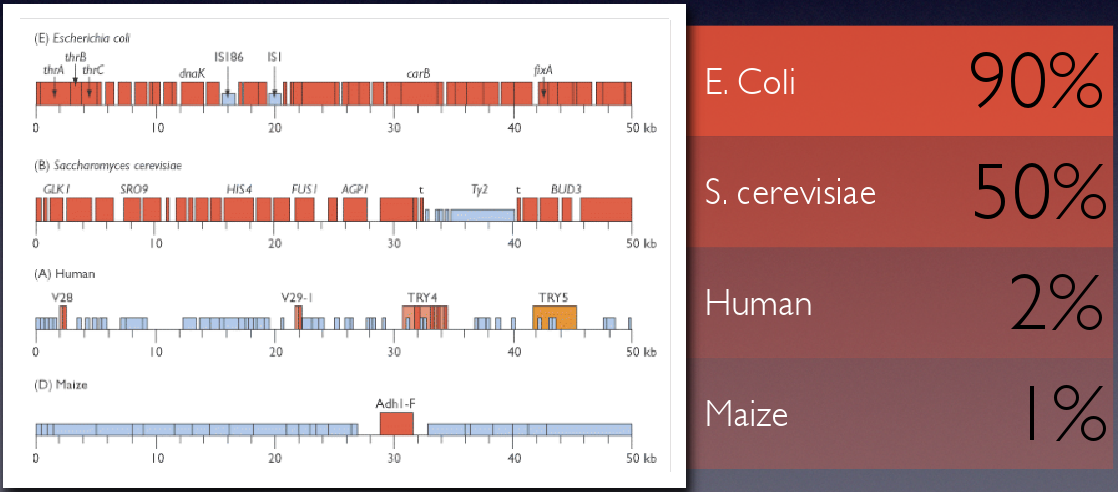
\includegraphics[width=0.95\textwidth]{img/genes}
\end{center}
\end{frame}

\begin{frame}
\frametitle{Genoma}
\framesubtitle{¿Para que sirve?}
\begin{columns}
\begin{column}{0.7\textwidth}
\begin{itemize}
    \item \textbf{Diagnóstico} y \textbf{prevención} de enfermedades\\
%    \begin{itemize}
%        \item Prueba genética
%%las pruebas basadas en el ADN son casi el primer uso
%%comercial y de aplicación médica de los nuevos descubrimientos en genética.
%%Estos ensayos se pueden usar para el diagnóstico de enfermedades, la
%%confirmación diagnostica, la información del pronóstico así como del curso de
%%la enfermedad, para confirmar la presencia de enfermedad en pacientes
%%asintomáticos y, con variados grados de certeza, para predecir el riesgo de
%%enfermedades futuras en personas sanas y en su descendencia.
%    \end{itemize}
    \item Estudio de \textbf{susceptibilidad} en las enfermedades
    \item Intervención (\textbf{tratamiento}) sobre la enfermedad.
    \begin{itemize}
        \item Enfermedades hereditarias.
        \item La ``terapia génica''.
        \item Fármacos a la medida.
    \end{itemize}
\end{itemize}
\end{column}
\begin{column}{0.3\textwidth}
	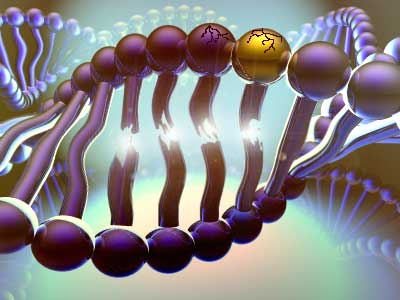
\includegraphics[width=0.95\textwidth]{img/autismo.jpg}
\end{column}
\end{columns}
\end{frame}

\begin{frame}
\frametitle{Genoma}
\framesubtitle{Otros Beneficios...}
\begin{columns}
\begin{column}{0.6\textwidth}
\begin{itemize}
    \item Medicina molecular.
    \item Genómica microbiana.
    \item Valoraciones de riesgo.
    \item Bioarqueología, antropología, \textbf{evolución}...
    \item \textbf{Identificación} ADN.
    \item \textbf{Agricultura} y \blue{bioprocesamiento}.
\end{itemize}
\end{column}
\begin{column}{0.4\textwidth}
	\begin{center}
		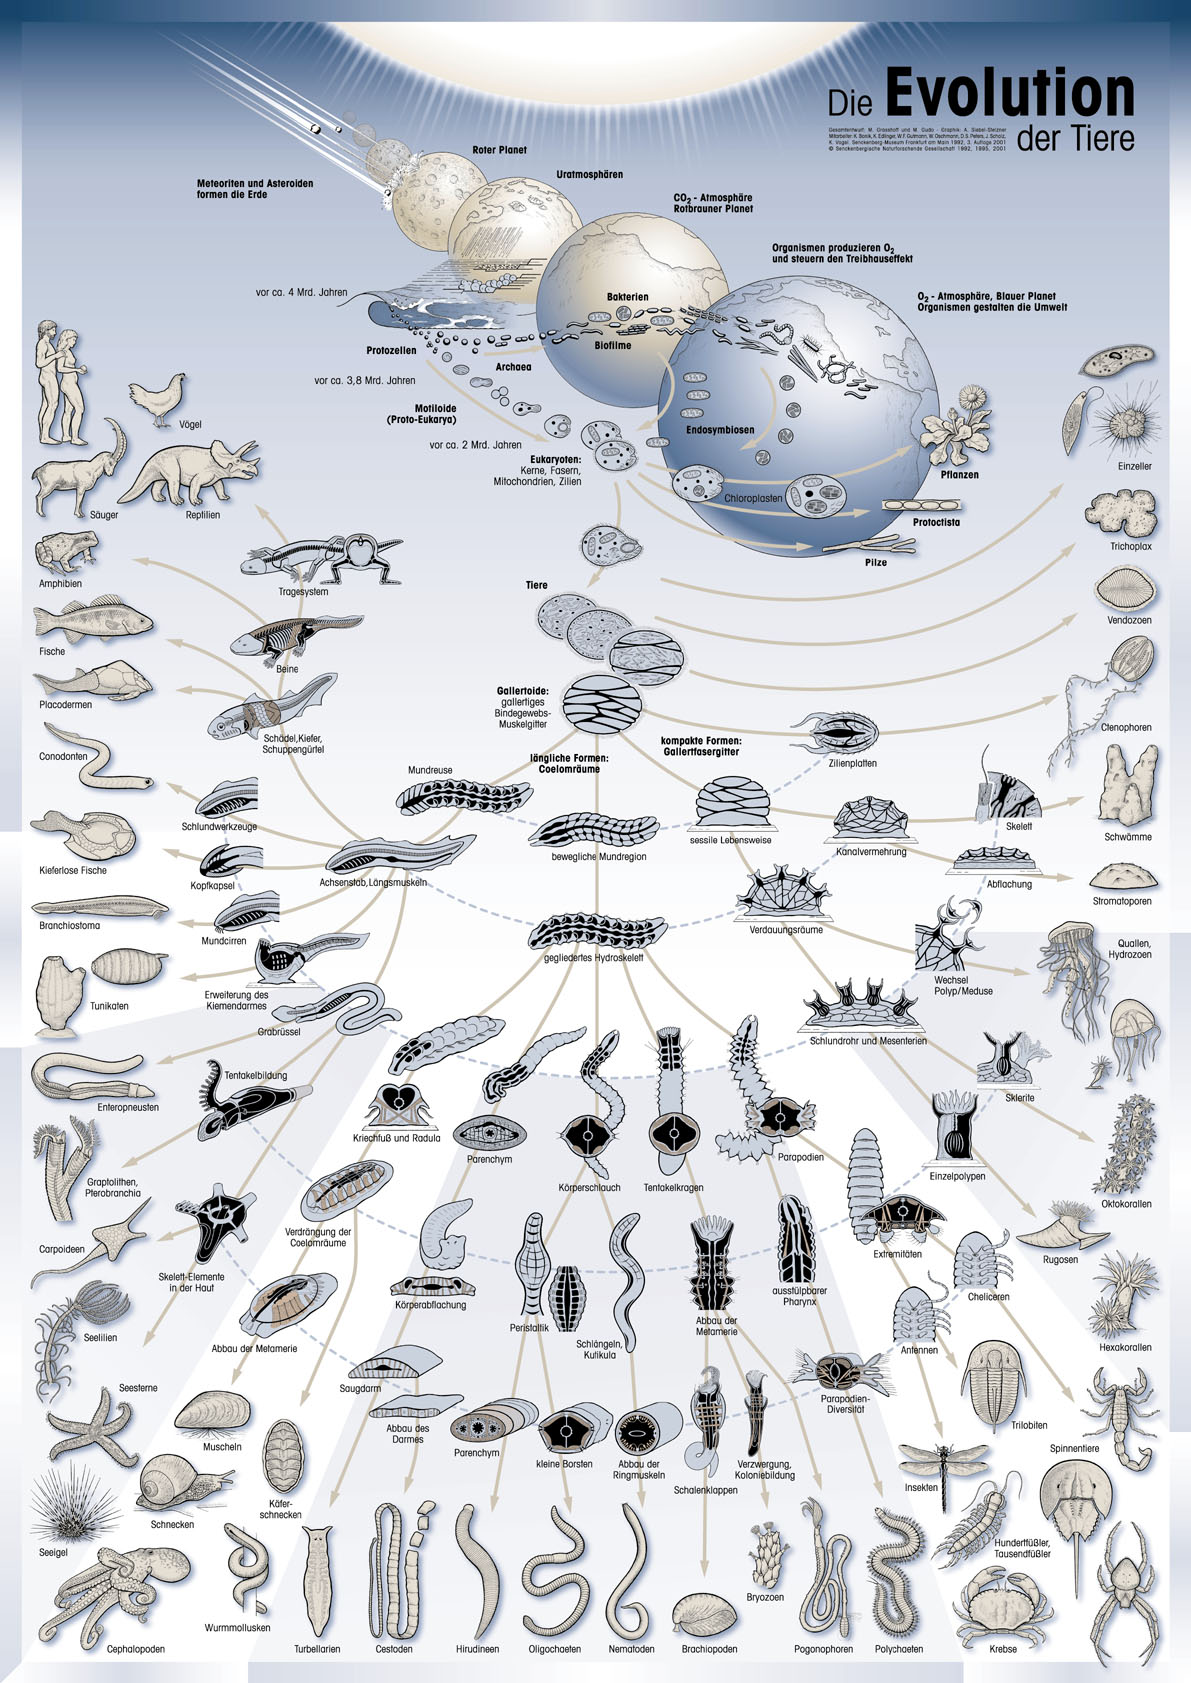
\includegraphics[width=0.95\textwidth]{img/evolution.jpg}
	\end{center}
\end{column}
\end{columns}
\end{frame}

\begin{frame}
\frametitle{Genoma}
\framesubtitle{Eucariotas}

\begin{columns}
\begin{column}{0.5\textwidth}
	\begin{itemize}
	    \item Uno o más \textbf{cromosomas} de DNA lineal.
	    \item De cada cromosoma, un par en cada célula.
	    \item Todos contenidos en el \textbf{núcleo}.
	    \item Los \textbf{genes} (codificando proteínas) ocupan un porcentaje pequeño del
	        DNA.
	    \item Los genes suelen estar interrumpidos por \textbf{intrones}.
	    \item \textbf{Mayor tamaño} que en los procariotas.
	\end{itemize}
\end{column}
\begin{column}{0.5\textwidth}
	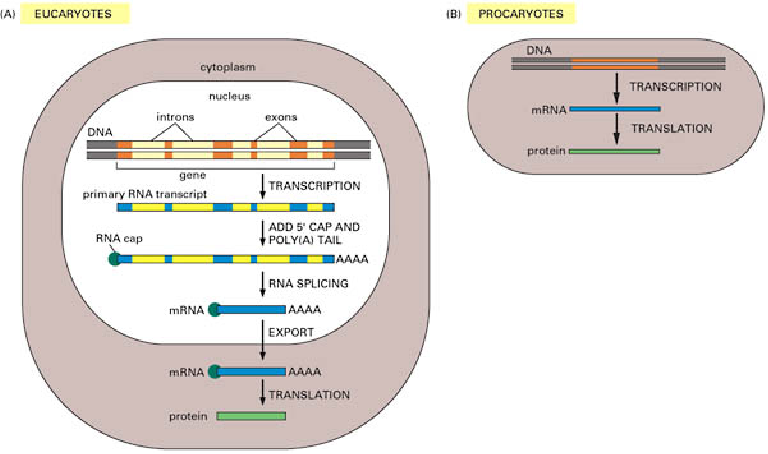
\includegraphics[width=0.95\textwidth]{img/eucariota_procariota}
\end{column}
\end{columns}
\end{frame}

\begin{frame}
\frametitle{Genoma}
\framesubtitle{Procariotas}
\begin{columns}
\begin{column}{0.5\textwidth}
\begin{itemize}
    \item Doble hélice Circular.
    \item \textbf{Flota} ``por ahí''.
    \item Suelen haber \textbf{plásmidos}.
\end{itemize}
\end{column}
\begin{column}{0.5\textwidth}
	\begin{center}
		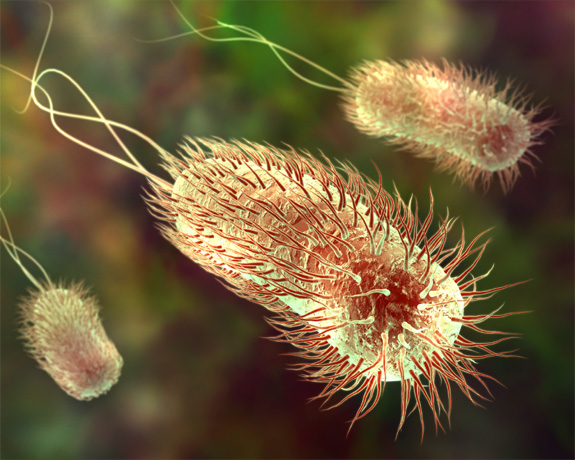
\includegraphics[width=0.95\textwidth]{img/procariota.jpg}
	\end{center}
\end{column}
\end{columns}
\end{frame}

\begin{frame}
\frametitle{Genoma Humano}
\framesubtitle{Algunos datos}
\begin{columns}
\begin{column}{0.7\textwidth}
	\begin{itemize}
	    \item \textbf{38.000} genes (app. \textbf{2\%} de todo el genoma).
	    \item 98\% idéntico al de los \textbf{chimpancés} y otros primates. 99,99\% de
	    similitud entre seres humanos. 
	    \item Se han encontrado 223 genes humanos que resultan similares a los
	    genes \textbf{bacterianos}. (hasta ahora)
	    \item \textbf{5 \%} del genoma codifica \textbf{proteínas}.
	\end{itemize}
\end{column}
\begin{column}{0.3\textwidth}
\begin{center}
	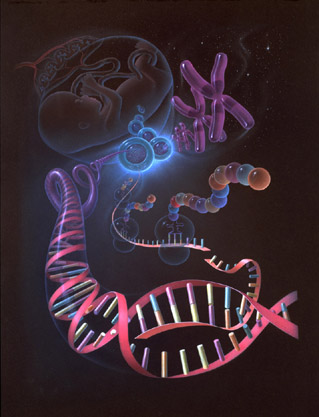
\includegraphics[width=0.95\textwidth]{img/genoma_humano.jpg}\\
\end{center}
\end{column}
\end{columns}
\end{frame}

\begin{frame}
\frametitle{Genoma Humano}
\framesubtitle{Algunos datos}
\begin{columns}
\begin{column}{0.7\textwidth}
	\begin{itemize}
	    \item  El \textbf{25\%} del genoma humano está casi \textbf{desierto}, existiendo largos espacios libres entre un gen y otro.
	    \item \textbf{35\%} + del genoma contiene secuencias \textbf{repetidas} (ADN basura)
	    \item \textbf{250-300.000} proteínas distintas.
	    \begin{itemize}
	        \item Por tanto cada gen podría estar
	        implicado por término medio en la síntesis de unas \textbf{diez} proteínas.
	    \end{itemize}
	    \item Entre \textbf{1,4 a 2,1} millones de variaciones de un sólo
        nucleótido en el genoma. (hasta ahora)
	\end{itemize}
\end{column}
\begin{column}{0.3\textwidth}
	\begin{center}
		
\includegraphics[width=0.95\textwidth]{img/genoma-humano.jpg}
	\end{center}
\end{column}
\end{columns}
\end{frame}


\begin{frame}
\frametitle{Genoma}
\framesubtitle{Información General}
\begin{columns}
\begin{column}{0.7\textwidth}
	\begin{itemize}
	    \item El récord en tamaño de genoma lo tiene la \textbf{ameba}, con
	    \textbf{670 Gbp} (versus 3 Gbp del
	humano).
	    \item El récord de \textbf{cantidad de genes} va para un cierto
	    \textbf{protozoo}, con \textbf{60.000} (el
		triple que nosotros).
	\end{itemize}
\end{column}
\begin{column}{0.3\textwidth}
\begin{center}
	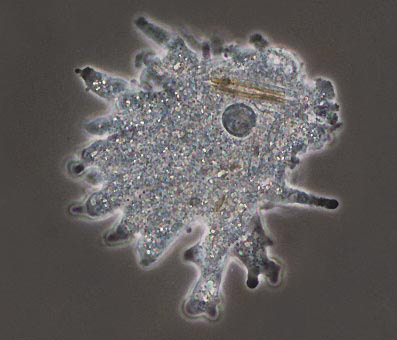
\includegraphics[width=0.95\textwidth]{img/ameba.jpg}
\end{center}
\end{column}
\end{columns}
\end{frame}

\begin{frame}
\frametitle{Genoma}
\framesubtitle{Información General}
\begin{center}
	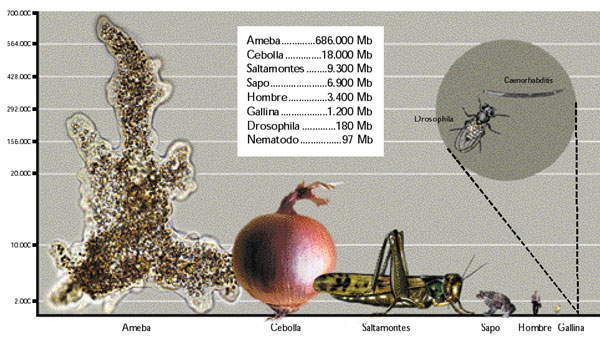
\includegraphics[width=0.95\textwidth]{img/tamanos.jpg}
\end{center}
\end{frame}

\begin{frame}
\frametitle{Genoma}
\framesubtitle{Información General 2}
\begin{columns}
\begin{column}{0.7\textwidth}
	\begin{itemize}
	    \item Las \textbf{vacas} tienen \textbf{60} cromosomas; el \textbf{pez
	    dorado}, alrededor de \textbf{100}.
	    \item Lo único que sí es cierto es que en \textbf{procariotas} el tamaño
	    oscila \textbf{entre 1 y 100} Mbp.
	    \item Y que las cosas que \textbf{vuelan} suelen tener genomas
	    relativamente \textbf{pequeños}.
	\end{itemize}
\end{column}
\begin{column}{0.3\textwidth}
\begin{center}
	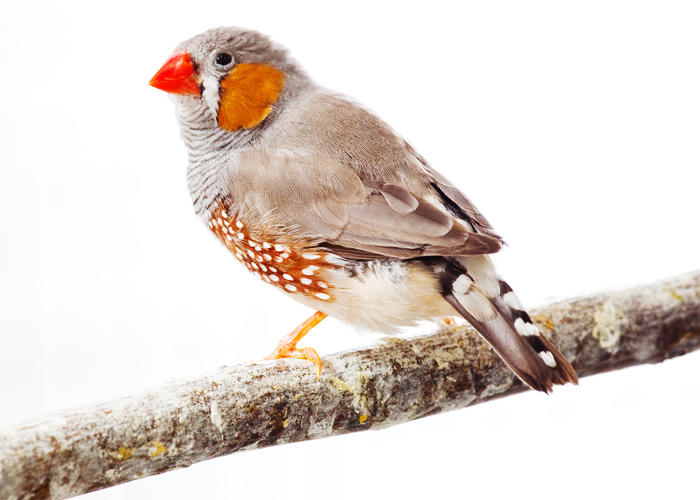
\includegraphics[width=0.95\textwidth]{img/ave.jpg}\\
\end{center}
\end{column}
\end{columns}
\end{frame}

\begin{frame}
\frametitle{Genoma}
\framesubtitle{Información General 3}
\begin{center}
	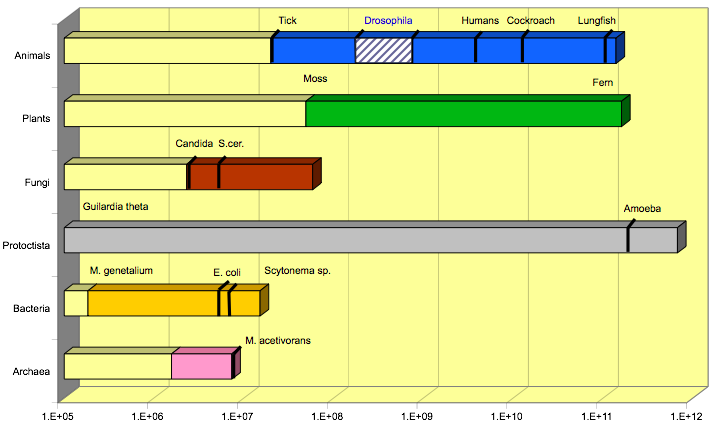
\includegraphics[width=0.95\textwidth]{img/gen_clados}
\end{center}
\end{frame}
